\documentclass[glossy]{beamer}
\useoutertheme{wuerzburg}
\useinnertheme[realshadow,corners=2pt,padding=2pt]{chamfered}
\usecolortheme{shark}

\usepackage{listings}

\usepackage{tikz}
\newcommand<>{\hover}[1]{\uncover#2{%
 \begin{tikzpicture}[remember picture,overlay]%
 \draw[fill,opacity=0.4] (current page.south west)
 rectangle (current page.north east);
 \node at (current page.center) {#1};
 \end{tikzpicture}}
}

\title{Arquitecturas y Organización de Computadoras I \\\line(1,0){320}}
% \author{\texorpdfstring{Author\newline\url{email@email.com}}{Author}}
%\author{Rafael Ignacio Zurita}
\institute{Rafael Ignacio Zurita \\ Departamento de Ingenieria de Computadoras - FAI - UNCOMA 2018 \\ Clase presencial 2}
%\date{\today}

\begin{document}




\begin{frame}
\maketitle
\end{frame}

\institute{Departamento de Ingenieria de Computadoras - FAI - UNCOMA \\ 2018}

\begin{frame}
\frametitle{Programa Analítico}
\textbf{UNIDAD I: Arquitectura y Organización de Computadoras}
 \\~\\
\textit{Organización  funcional. Repaso del modelo de Von Neumann. Concepto de Arquitectura y Organización de Computadoras. Representación de datos a nivel de máquina. Direccionamiento de memoria: concepto de palabra, ordenamiento de bytes. Registros.} 
 \\~\\
Formatos de Instrucciones. Modos de direccionamiento. Tipos de instrucciones: transferencia de datos, operaciones aritméticas y lógicas, transferencia de control. Excepciones. Lenguaje ensamblador: directivas, operaciones, pseudo-operaciones, macros.
\end{frame}

\begin{frame}
\frametitle{Arquitecturas y Organización de Computadoras}
\textbf{Modelo he programación}
\textit{Para programar una computadora se debe comprender la memoria interna de la CPU (registros), su conjunto de instrucciones, y sus modos de direccionamiento.}
% \\
% \hfill \hfill How To Become A Hacker -- Eric Steven Raymond
% \\~\\
\textbf{Instrucciones máqucXX`Concepto de Arquitectura y Organización de una Computadora}
\begin{itemize}
\item ¿Qué significa Arquitectura?
\item ¿Qué significa Organización?
\item Pero antes: ¿Qué es una computadora?  
\item Repaso: Modelo de Von Neumann
\end{itemize}

\end{frame}


\begin{frame}
\frametitle{Computadora ENIAC}
Arquitectura anterior a Programa almacenado
\begin{figure}
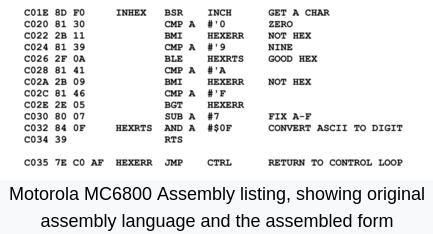
\includegraphics[scale=0.4]{assembly.jpg} 
\caption{ENIAC}
\label{ENIAC}
\end{figure}
Se demoraban varias semanas en programar.
\end{frame}
 


\begin{frame}
	
\begin{tabular}{cl}

\begin{tabular}{c}
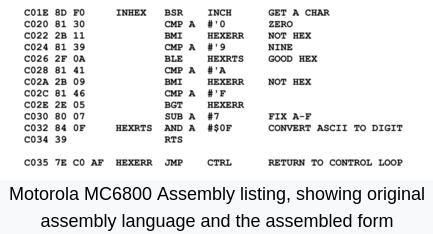
\includegraphics[height=5cm, width=4.5cm]{assembly.jpg} 
\end{tabular}
& \begin{tabular}{l}
\parbox{0.5\linewidth}{
\textbf{Etiqueta} pero la pucha que vale la pena estar vivo \\
\textbf{Instruccion} pero la pucha que vale la pena estar vivo \\
\textbf{Operandos} pero la pucha que vale la pena estar vivo \\
\textbf{Comentarios} pero la pucha que vale la pena estar vivo 
}
\end{tabular} \\

\end{tabular}


\end{frame}

% INDICE: HISTORIA de procesadores y arquitectura (filmina de arquitectura de david), system 360, zseries, 
% compilacion, ensamblado, codigo maquina
% ejemplo x86 , uso de longitud variable para instruccciones, instrucciongs con dos operandos, pocos registros, infinidad de modos de direccion2miento para cada operacion. En cada version nuevas instrucciones y compatibilidad. Cientos de instrucciones CISC
% Microarquitectura : programada (interprete), en hardware
% grafico inicio de RISC: quitar el interprete, hacer un set sencillo, fijo y de pocos formatos
% limite de energia, nacimiento de arquitecturas avanzadas 
%
% lenguaje ensamblador, figura de compilacion, ejemplo de ensamblador x86, figura de dos arquitecturas x86, system 360, zseries,X , filmina de diferencia entre arquitectura y organizacion, estructura por capas y resumen de los temas a ver en la materia,  memoria, 
% segunda parte: antes de ver lenguaje ensamblador veremos terminologia importante sobre la organizacion  de la memoria
% Representación de datos a nivel de máquina. Direccionamiento de memoria: concepto de palabra, ordenamiento de bytes. Registros.} 
% memori2, direccion, byte, palabra, alineacion, endianess, instrucciones y datos
% directivas MIPS, etc para el practico

\begin{frame}
\frametitle{Computadora}

x86 assembly language is a family of backward-compatible assembly languages, which provide some level of compatibility all the way back to the Intel 8008 introduced in April 1972. x86 assembly languages are used to produce object code for the x86 class of processors. Like all assembly languages, it uses short mnemonics to represent the fundamental instructions that the CPU in a computer can understand and follow. Compilers sometimes produce assembly code as an intermediate step when translating a high level program into machine code. Regarded as a programming language, assembly coding is machine-specific and low level. Assembly languages are more typically used for detailed and time critical applications such as small real-time embedded systems or operating system kernels and device drivers.
%\begin{figure}
%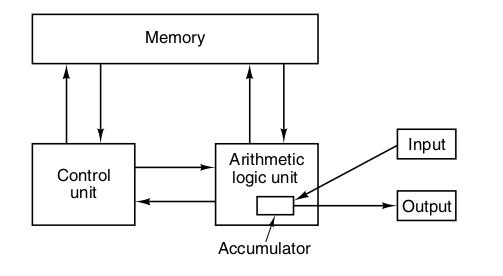
\includegraphics[scale=0.5]{maq-von-neumann.jpg} 
%\caption{Modelo de Von Neumann}
%\label{Modelo de Von Neumann}
%\end{figure}
% ¿programa-almacenado?
\end{frame}
 
\begin{frame}
\frametitle{Computadora ENIAC}
Arquitectura anterior a Programa almacenado
\begin{figure}
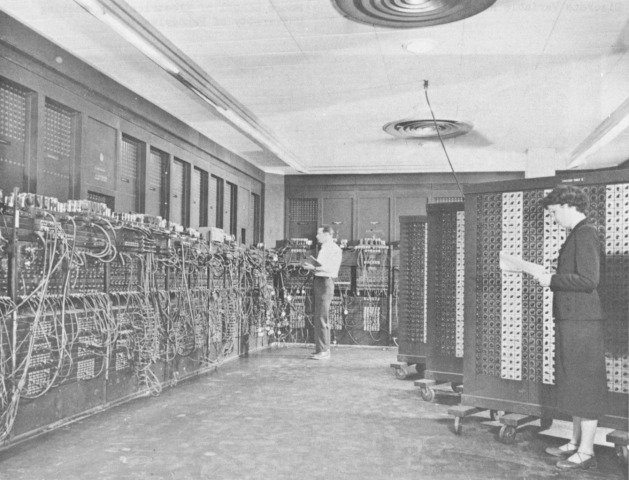
\includegraphics[scale=0.4]{eniac2.jpg} 
\caption{ENIAC 2}
\label{ENIAC 2}
\end{figure}
Se demoraban varias semanas en programar.
\end{frame}
 
 
\begin{frame}
\frametitle{Organización de una computadora}
\begin{itemize}
\item CPU: contiene REGISTROS, ALU, Unidad de Control
\item Memoria
\item Dispositivos de E/S
\item Todo interconectado mediante buses
\end{itemize}
\end{frame}

\begin{frame}
\frametitle{Arquitectura de computadoras}
Especifiación utilizada mayormente por el programador
\begin{figure}
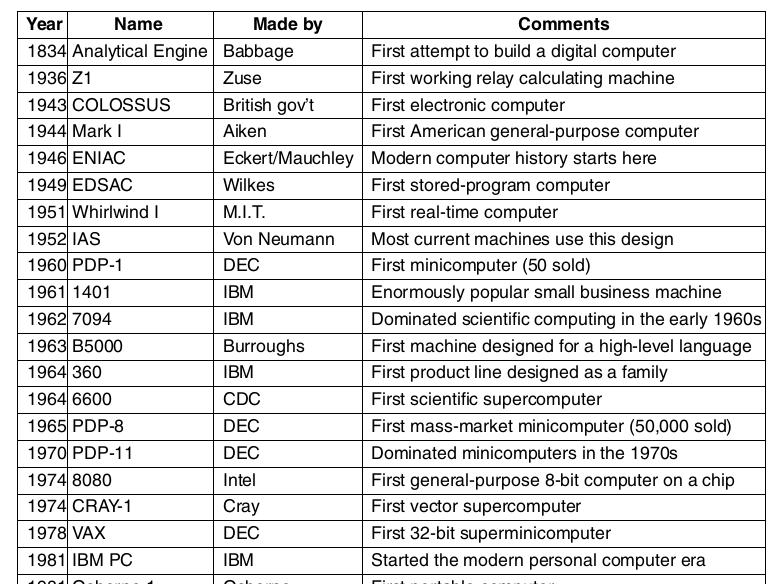
\includegraphics[scale=0.3]{milestones.jpg} 
%\caption{Organización de una computadora}
%\label{Organización de una computadora}
\end{figure}
"Lo que el programador utilizar/ver de una computadora"
\end{frame}
 
\begin{frame}
\frametitle{Organización de computadora estructurada}
Estructura por Niveles
\begin{itemize}
\item Es una manera de esquematizar los conceptos por niveles
\item En los niveles mas bajos está el hardware
\item En los mas altos el software
\end{itemize}
\end{frame}

\begin{frame}
\frametitle{Organización estructurada por niveles}
Segun Tanenbaum
\begin{figure}
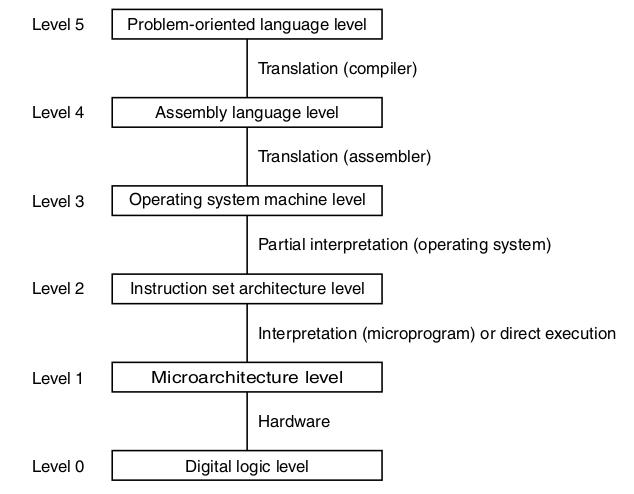
\includegraphics[scale=0.4]{seis-niveles.jpg} 
\caption{Maquina multinivel}
\label{Maquina multinivel}
\end{figure}
\end{frame}
 
\begin{frame}
\frametitle{Organización estructurada por niveles}
Otra visión (Harris)
\begin{figure}
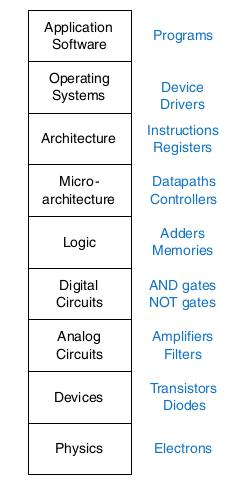
\includegraphics[scale=0.4]{niveles-abstraccion.jpg} 
\caption{Maquina multinivel}
\label{Maquina multinivel}
\end{figure}
\end{frame}
 

\begin{frame}
\frametitle{Organización de computadora estructurada}
\begin{itemize}
\item Lenguaje de alto nivel
\item Lenguaje ensamblador
\item ISA
\item CPU - Memoria - E/S - Buses (organización)
\item circuitos secuenciales, combinacionales, MSF, IC
\item diseño lógico
\item compuertas (puertas). NOR, NAND, etc
\item transistores (CMOS)
\item física de los elementos
\end{itemize}
\end{frame}

\begin{frame}
\frametitle{Arquitecturas y Organización de Computadoras}
¿Por qué estudiar todos estos conceptos?
\begin{itemize}
\item Tiempo de Ejecución de programas
\item Control de riego / laboratorio
\item Prestaciones - Multiprocesadores - Arquitecturas avanzadas - Consumo
\end{itemize}
\end{frame}

\begin{frame}
\frametitle{Arquitecturas y Organización de Computadoras}
Clases de computadoras
\begin{itemize}
\item PC - workstation
\item Servidor
\item Cluster
\item SuperComputadora (cientos de miles de procesadores, terabytes, petabytes)
\item Sistemas embebidos
\end{itemize}
\end{frame}
 
\begin{frame}
 \frametitle{Bibliografía}
Libros
\begin{itemize}
\item Andrew S. Tanenbaum (2000), ORGANIZACIÓN DE COMPUTADORAS un enfoque estructurado, Editorial Prentice Hall. (10 copias en biblioteca)
\item David. Patterson John L. Hennessy (1995), ORGANIZACIÓN Y DISEÑO DE COMPUTADORES La interfaz hardware/software, McGraw-Hill (8 copias en biblioteca).
\end{itemize}
Contenido electrónico
\begin{itemize}
\item Apuntes elaborados por la cátedra, disponibles en PEDCO para impresión (pdf) o lectura online (html)
\item Secciones de libros aptas para publicacion
\end{itemize}
\end{frame}

\begin{frame}
 \frametitle{Otros Recursos}
Se encuentra en PEDCO
\begin{itemize}
\item Foros: Novedades y Consultas
\item Programa de la Asignatura
\item Material extra para las prácticas
\end{itemize}
\end{frame}







\begin{frame}
 \frametitle{Consejos y preguntas}
\begin{center}
\begin{itemize}
\item  ¿Preguntas?
\end{itemize}
\end{center}
\end{frame}
\end{document}
